\subsection{Meta Surfaces}

\subsection{The S-Matrix Formalism}

\begin{equation}
    \hat{S} =
    \begin{pmatrix}
        \hat{T}^f & \hat{R}^b \\
        \hat{R}^f & \hat{T}^b
    \end{pmatrix}
\end{equation}


\subsection{SASA and the Star Product}


\subsection{(Convolutional) Neural Networks}
Artificial Neural Networks (ANN's or short NN's) are a kind of data structure inspired by the biological Neurons found in Nature. They can be used to find a wide range of input output relations. One classic example is mapping pictures of hand written digits to the actual digits. Rather then explicitly program the relation NN's are trained on a dataset $(X, \, Y)$ of correct input output pairs.
\\


\begin{figure}[H]
    \centering
    \includegraphics[width=.6\linewidth]{bg_basic_nn}
    \caption{The most simple kind of NN is called densely connected. For clarity only connections to the top most nodes of each layer are shown.}
    \label{fig:bg:basic_nn}
\end{figure}

\paragraph{Densely Connected Neural Networks}
This kind of NN consist of single nodes which are organized into layers. Every node is connected to all the nodes of the previous and next layer thus they are called dense. Each node holds a value called activation $a$ where the activation to the first layer is the input to the network, here:
$(x_1, \, x_2, \, x_3)$.
To calculate the activation of a node one has to multiply all the previous activations with their respective weights $w$, add the bias $b$ and finally apply a non-linear activation function $\sigma$. For the index notation superscripts specify the layer and subscripts the node. So $a^2_1$ is the activation of the first node in the second layer. To characterize a weight two subscripts are needed for the end and beginning of the connection. For the example in \ref{fig:bg:basic_nn} that means:

\begin{equation} \label{eq:bg:activation_example}
    a^2_1 = \sigma \qty(\sum_i w^2_{1i} \, x_i + b^2_1)
\end{equation}

\noindent
However it is more convenient to stop considering every node individually and to view the involved quantities as vectors and matrices. So that \eqref{eq:bg:activation_example} can be written as:

\begin{equation} \label{eq:bg:activation}
    \vb{a}^l = \sigma \qty(\vu{w}^l \vb{a}^{l-1} + \vb{b}^l)
\end{equation}

\begin{figure}[H]
\centering
\begin{subfigure}{.5\textwidth}
    \centering
    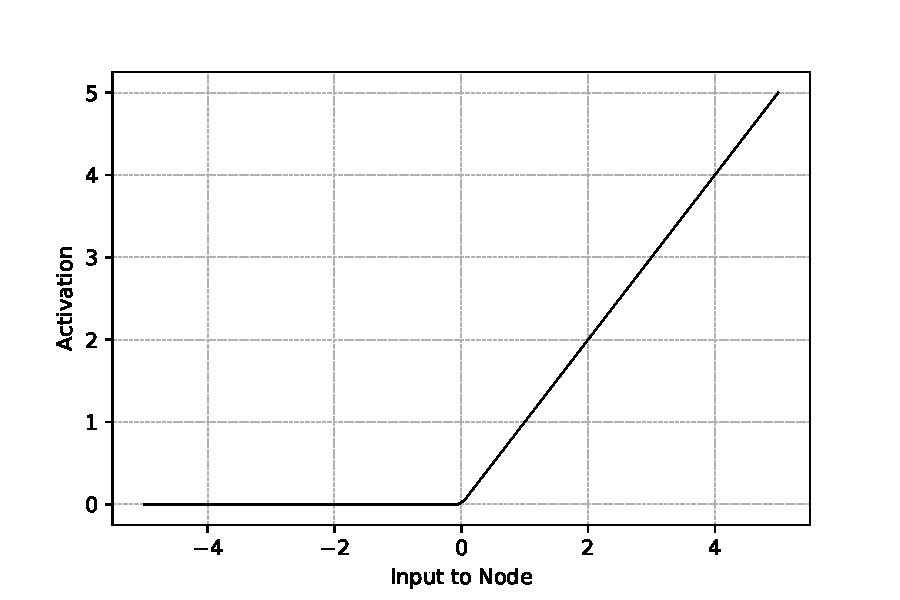
\includegraphics[width=\linewidth]{bg_relu}
    \caption{relu}
    \label{}
\end{subfigure}%
\begin{subfigure}{.5\textwidth}
    \centering
    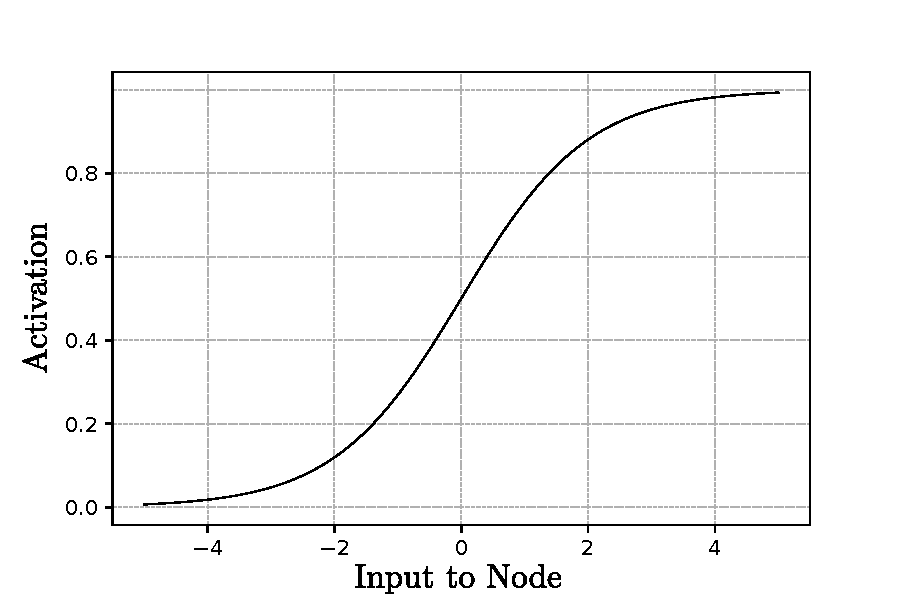
\includegraphics[width=\linewidth]{bg_sigmoid}
    \caption{sigmoid}
    \label{}
\end{subfigure}
\caption{Two examples of activation functions $\sigma$.}
\label{}
\end{figure}

\paragraph{Training}
During training the network output $\s{NN}(\vb x) = \vb{y}' $ is calculated though repeated use of \eqref{eq:bg:activation} and is then compared with the known correct output $\vb y$ by a cost function $C = C(\vb y, \, \vb y')$. This might simply be the mean squared difference between $\vb y$ and $\vb y'$ but there are more sophisticated cost functions for different kind of outputs. Now we can quantify how well the NN is performing but how should the weights and biases be changed to improve this performance?
Here a very important Algorithm \textit{Backpropagation} comes into play and allows a efficient calculation of $\grad{C}_{\vb{b}^l}$ and $\grad{C}_{\vu{w}^l}$. These are used to gradually minimize the cost function. A very comprehensive explanation of Backpropagation can be found here: \cite{backprop}.

\paragraph{Convolutional Neural Networks}
